\subsubsection{Category}\label{subsec:appendix_category}
There are $58$ different category labels present within the dataset.
Categories with less than 140 documents ($0.1\%$ of the number of documents) are removed as part of preprocessing and replaced with a single miscellaneous category 'misc'.
This reduces the number of categories to $34$, while only replacing 292 documents to have the 'misc' category.
This preprocessing also makes the size of the remaining categories more evenly distributed, as can be seen in \autoref{fig:category_hist}.

\begin{figure*}[ht]
	\centering
	\begin{subfigure}{0.45\textwidth}
		\centering
		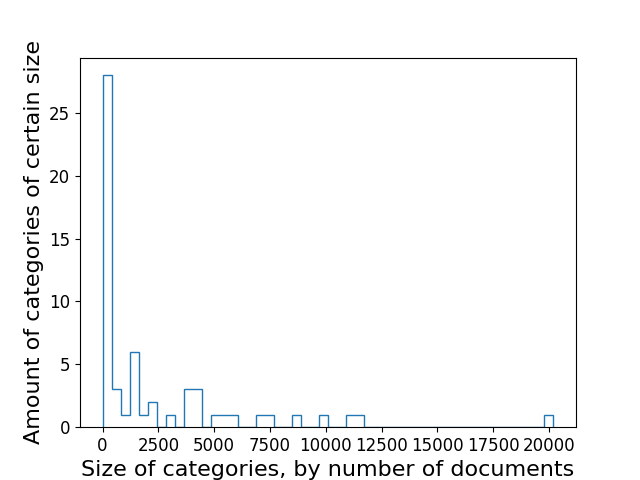
\includegraphics[width=\linewidth]{figures/category_hist2_before.png}
		\caption{Before preprocessing}
		\label{fig:category_hist_before}
	\end{subfigure}
	\begin{subfigure}{0.45\textwidth}
		\centering
		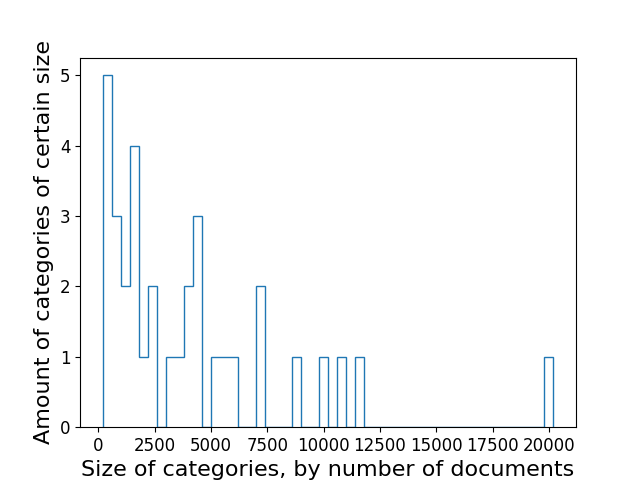
\includegraphics[width=\linewidth]{figures/category_hist2_140.png}
		\caption{After preprocessing}
		\label{fig:category_hist_after}
	\end{subfigure}
	\caption{Histogram over the number of categories for different number of documents, before and after preprocessing.
	Categories on the x-axis are grouped into 50 buckets.}
	\label{fig:category_hist}
\end{figure*}

As mentioned in \autoref{sec:dataset}, there are some category labels which seemingly have no relevance to the documents using the labels.
Specifically, the category labels '26. Frederik' and '53. Frederik' do not indicate what they cover, since Frederik is simply a normal Danish name.
Since they are not filtered into the 'misc' category during preprocessing, it is worth looking into what documents have these categories.

By looking at a random selection of documents from these categories, there is no clear pattern to be found.
The topics, within these categories, can be about anything from sports to news from anywhere around the world or locally in Denmark.
The articles from '26. Frederik' appear all years in our dataset, while the articles for '53. Frederik' seem to be just from 2019, the last year in our dataset, but evenly distributed over the whole year.
Curiously enough, most of the documents from these categories seem to be written by Anders Kjærgaard, with only a few other authors.
For '26. Frederik' there are just 5 unique authors: Carsten Tolbøll, Emil Abkjær Kristensen, Morten Kyndby Holm, Jens Fogh-Andersen, and Anders Kjærgaard.
For '53. Frederik' there are just 4 unique authors: Klaus Færch Gjerulff, Morten Kyndby Holm, Jens Fogh-Andersen, and Anders Kjærgaard.
This shows that Morten Kyndby Holm, Jens Fogh-Andersen, and Anders Kjærgaard have written for both categories.

\vejleder[inline]{what happens if you merge them?}
From the exploration of these two categories, we can not say with certainty why these categories exist, or why multiple authors have chosen to write for these categories.
We continue to use these categories in our experiment, for the possibility of making other observations through the topic models.

\begin{table*}[h]
	\caption{Number of documents for each of the 58 categories within the Nordjyske dataset from 2017 to 2019.
		The highlighted categories are filtered and combined during preprocessing.}
	\label{tab:category_table}
	\centering
	\begin{tabular}{l|c|l|c|l|c|l|c}
		Category            & Number & Category        & Number & Category                       & Number & Category                    & Number \\
		\midrule
		Fælles              & 20204  & Navne           &  3749  & Kram                           &  244   & \textbf{Østvendsyssel Avis} &   4    \\
		Thisted-avis        & 11473  & Kultur          &  3012  & 53. Frederik                   &  203   & \textbf{DF Motor Biler}     &   3    \\
		Sport-avis          & 10941  & Morsø Sport     &  2350  & Feature                        &  188   & \textbf{Nyhedsmotoren-net}  &   3    \\
		Debat               & 10075  & Friii           &  2333  & \textbf{Aalborg:nu}            &   73   & \textbf{Plus Publicering}   &   3    \\
		Udland-avis         &  8855  & Bagside         &  1933  & \textbf{Erhvervsnavne}         &   39   & \textbf{RB}                 &   3    \\
		Erhverv-avis        &  7356  & MitLiv          &  1519  & \textbf{Newspack}              &   35   & \textbf{Sport-net}          &   3    \\
		Mariagerfjord-avis  &  7241  & WEEKEND         &  1493  & \textbf{DF Søfart}             &   32   & \textbf{Thisted-net}        &   3    \\
		Morsø-avis          &  5959  & Bo Godt         &  1447  & \textbf{Morsø Ugeavis}         &   27   & \textbf{Hanbo-bladet}       &   2    \\
		Aalborg-avis        &  5544  & Nordjyske Biler &  1400  & \textbf{DF Licitation Byggeri} &   14   & \textbf{Brugermappe}        &   1    \\
		Vesthimmerland-avis &  5131  & Morsø Debat     &  1375  & \textbf{Biler}                 &   13   & \textbf{Brønderslev-net}    &   1    \\
		Rebild-avis         &  4415  & Frieord         &  1341  & \textbf{Samfund}               &   9    & \textbf{Lokalavisen}        &   1    \\
		Frederikshavn-avis  &  4325  & Indsigt         &  984   & \textbf{Nordjyske Plus}        &   6    & \textbf{Mariagerfjord-net}  &   1    \\
		Hjørring-avis       &  4235  & Thisted sport   &  698   & \textbf{Oplandsavisen}         &   6    & \textbf{Morsø-net}          &   1    \\
		Brønderslev-avis    &  3857  & Perspektiv      &  613   & \textbf{INFOMAKER PRINT}       &   5    &                             &        \\
		Jammerbugt-avis     &  3791  & 26. Frederik    &  484   & \textbf{DF Licitation Diverse} &   4    &                             &        \\
		\bottomrule
	\end{tabular}
\end{table*}
